Recurrent neural networks differ from feed forward neural networks because of the presence of recurrent connections: at least one perceptron output at a given layer $i$ is \textit{fed} to another perceptron
at a level $j<i$, as can be seen in figure \ref{rnn_model}. 
This is a key difference, as we will see in later sections, because it introduces \textit{memory} in the network, changing, somehow, the expressiveness
of the model.


\tikzstyle{rnn_style}=[->,shorten >=1pt,auto,node distance=1.5cm,
  thick,
  neuron/.style={circle,fill=white!50,node distance =1.2cm,draw,minimum size=0.7cm,font=\sffamily\Large\bfseries},
  missing/.style={rectangle,node distance =1.2cm,fill=white!50,draw=none,minimum size=0.7cm,font=\sffamily\Huge\bfseries},
  label/.style={node distance=1.2cm,rectangle,fill=white!50,draw=none,minimum size=0.7cm,font=\sffamily\normalsize},
  layer/.style={rectangle,fill=white!50,draw,minimum width=4cm,font=\sffamily\normalsize},
  loopStyle/.style={in=120,out=60, distance=2.5cm},]
\begin{figure}[!h]
 \centering
\begin{tikzpicture}[rnn_style]

  \node[neuron]    (x0)       {};
  \node[neuron]    (x1)[right of=x0]   {};
  \node[neuron]    (x2)[right of=x1]   {};
  \node[missing]   (x3)[right of=x2]   { $\hdots$};
  \node[neuron]    (xn)[right of=x3]   {};
  
  \node[label]    (u0)[below of=x0]   {$u_0[t]$};
  \node[label]    (u1)[below of=x1]   {$u_1[t]$};
  \node[label]    (u2)[below of=x2]   {$u_2[t]$};
  \node[label]    (un)[below of=xn]   {$u_n[t]$};
  
  
  \node[layer] (hl)[above of=x2,node distance=2cm] {Hidden layer};
  \node[neuron](b) [right of=hl,node distance=3cm] {};
  \node[label] (b_l) [right of=b] {bias=1};
  \node[layer] (ol)[above of=hl,node distance=2cm] {Output layer};
  
  \node[neuron] (o1) at (0,5.5) {};
  \node[neuron] (o2)[right of=o1] {};
  \node[neuron] (o3)[right of=o2] {};
  \node[missing](o4)[right of=o3] {$\hdots$};
  \node[neuron] (on)[right of=o4] {};
  
  
  \node[label]    (y0)[above of=o1]   {$y_0[t]$};
  \node[label]    (y1)[above of=o2]   {$y_1[t]$};
  \node[label]    (y2)[above of=o3]   {$y_2[t]$};
  \node[label]    (yn)[above of=on]   {$y_n[t]$};
  
  
  \path[->] (x0) edge [] node[]{$W_{in}$}   (hl)
	    (x1) edge []   (hl)
	    (x2) edge []   (hl)
	    (xn) edge []   (hl)
	    (u0) edge []   (x0)
	    (u1) edge []   (x1)
	    (u2) edge []   (x2)
	    (un) edge []   (xn)
	    (ol) edge []   (o1)
	    (ol) edge []   (o2)
	    (ol) edge []   (o3)
	    (ol) edge []   (on)
	    (o1) edge []   (y0)
	    (o2) edge []   (y1)
	    (o3) edge []   (y2)
	    (on) edge []   (yn)
	    (hl) edge []  node[]{$W_{out}$} (ol)
	    (b)  edge [bend left,dotted,in= 160]  node[]{$b_{rec}$} (hl)
	    (b)  edge [bend left,dotted,anchor=west, in= -160]  node[]{$b_{out}$} (ol)
	    (hl) edge [loop ,in=-160,out=160, distance=3cm,anchor=east ]      node [align=center]  {$W_{rec} $} (hl);

\end{tikzpicture}
\caption{$\net{RNN}$ model}
\label{rnn_model}
\end{figure}


This difference in topology reflects also on the network's input and output domain: where, in feed froward neural networks, inputs and outputs were real valued vectors, recurrent neural networks deal with
sequences of vectors; in other words time is also considered. One may argue that, taking time (and sequences) into consideration, is some sort of limitation, because it restricts our model to deal only
with temporal inputs; however that's not the case, in fact we can apply RNNs to non temporal data by considering space as the temporal dimension, for example imagine feeding the network with the pixels of an image one column at a time; or we can feed the network with the same input for all time steps or simply
providing no input at all after the first step.

\begin{defn}[Recurrent neural network]
\label{def_rnn}
A recurrent  neural network is tuple
$$\net{RNN}\defeq< \set{W},\set{B} ,\sigma(\cdot),F(\cdot)>$$
\begin{itemize}
 \item $\set{W} \defeq \{\mat{W}^{in},\mat{W^{rec},\mat{W^{out}}}\}$ where
 \begin{itemize}
  \item $W^{in}$ is the $r\times p$ input weight matrix
  \item $W^{rec}$ is the $r\times r$ recurrent weight matrix
  \item $W^{out}$ is the $o \times r$ output weight matrix
 \end{itemize}
 \item $\set{B} \defeq \{\vec{b^{rec},\vec{b^{out}}}\}$ where
 \begin{itemize}
   \item $\vec{b}^{rec} \in \mathbb{R}^{r}$ is the bias vector for the recurrent layer
   \item $\vec{b}^{out} \in \mathbb{R}^{o}$ is the bias vector for the output layer
 \end{itemize}
 \item $\sigma(\cdot): \mathbb{R}\rightarrow \mathbb{R}$ is the activation function
 \item $F(\cdot): \mathbb{R}^{o}\rightarrow \mathbb{R}^{o}$ is the output function
\end{itemize}
\end{defn}

\begin{remark}{}
Given a $\net{RNN}$
\begin{itemize}
 \item The total number of weights si given by $\mathcal{N}(W) \defeq rp+r^2+ro$
 \item The number of biases by $\mathcal{N}(b) \defeq r+o $
 \item $p$ is the size of input vectors, 
 \item$r$ is the number of hidden units
 \item $o$ is the size of output vectors. 
\end{itemize}
\end{remark}

\begin{defn}[Output of a $\net{RNN}$]
\label{def_rnn_output}
Given a $\net{RNN}$ and an input sequences $\{\vec{x}\}_{t=1,...,T}, \vec{x}_t \in \mathbb{R}^p$ the output sequence $\{\vec{y}\}_{t=1,...,T}, \vec{y}_t \in \mathbb{R}^o$ of the net is defined by the following:
\begin{align}
&\vec{y}^t \defeq F(W^{out}\cdot\vec{a}^t + \vec{b}^{out})\\
&\vec{a}^t \defeq W^{rec}\cdot\vec{h}^{t-1}+W^{in}\cdot\vec{x}^t+\vec{b}^{rec}\\
&\vec{h}^t \defeq  \sigma(\vec{a}^t) \\
&\vec{h}^0 \defeq \overrightarrow{0}
\end{align}
\end{defn}


As we can understand from definition \ref{def_rnn_output}, there is only one recurrent layer, whose weights are the same for each time step, so one could asks where does the deepness of the network come from.
The answer lies in the temporal unfolding of the network, in fact if we unfold the network step by step we obtain a structure similar to that of a feed forward neural network. As we can observe
in figure \ref{rnn_unfolding}, the unfolding of the network through time consist of putting identical version of the same recurrent layer one on top of each other and linking the inputs of one layer to the
next one. The key difference from feed forward neural networks is, as we have already observed, that the weights in each layer are identical; another
important unlikeness is of course the presence of additional timed inputs for each unfolded layer.

\tikzstyle{rnn_style}=[->,shorten >=1pt,auto,node distance=1.5cm,
  thick,
  neuron/.style={circle,fill=white!50,draw,minimum size=0.7cm,font=\sffamily\Large\bfseries},
  missing/.style={circle,fill=white!50,draw=none,minimum size=0.7cm,font=\sffamily\Huge\bfseries},
  label/.style={node distance=1.2cm,rectangle,fill=white!50,draw=none,minimum size=0.7cm,font=\sffamily\normalsize},
  layer/.style={rectangle,fill=white!50,draw,minimum width=4cm,font=\sffamily\normalsize},
  loopStyle/.style={in=120,out=60, distance=2.5cm},]
\begin{figure}[h!]
 \centering
\begin{tikzpicture}[rnn_style]

  %t=0
  \node[layer] (hl1) {Hidden layer t=0};
  
  \node[neuron]    (x0)[below left=0.3cm and 1cm of hl1]       {};
  \node[label]    (u0)[left of=x0]   {$\vec{x}_1$};
  

  
  \node[neuron] (o0) [above right=0.3cm and 1cm of hl1] {};
  \node[label]    (y0)[right of=o0]   {$\vec{y}_1$};
  
  %t=1
  \node[layer] (hl2)[above of=hl1,node distance=2.5cm] {Hidden layer t=1};
  
  \node[neuron]    (x1)[below left=0.3cm and 1cm of hl2]      {};
  \node[label]    (u1)[left of=x1]   {$\vec{x}_2$};
  
    
  \node[neuron] (o1) [above right=0.3cm and 1cm of hl2] {};
  \node[label]    (y1)[right of=o1]   {$\vec{y}_2$};
  
  %dots
  \node[label,font=\sffamily\Huge\bfseries] (hld)[above of=hl2,node distance=2cm] {$\hdots$};
  
  %t=T
  \node[layer] (hlT)[above of=hld,node distance=2cm] {Hidden layer t=T};
  
  \node[neuron]    (xT)[below left=0.3cm and 1cm of hlT]      {};
  \node[label]    (uT)[left of=xT]   {$\vec{x}_T$};
  
    
  \node[neuron] (oT) [above right=0.3cm and 1cm of  hlT] {};
  \node[label]    (yT)[right of=oT]   {$\vec{y}_T$};
  
  
  %biases
  \node[neuron](b) [right of=y1,node distance=1.4cm] {};
  \node[label] (b_l) [above of=b,node distance=0.7cm] {bias=1};

  
  \path[->] (x0) edge [bend right] node[]{$W^{in}$}   (hl1)
	    (u0) edge []   (x0)
	    (o0) edge []   (y0)
	    (x1) edge [bend right] node[]{$W^{in}$} (hl2)
	    (u1) edge []   (x1)
    	    (o1) edge []   (y1)
	    (xT) edge [bend right] node[]{$W^{in}$} (hlT)
	    (uT) edge []   (xT)
    	    (oT) edge []   (yT)

	    
	    (hl1) edge [bend left]  node[]{$W^{out}$} (o0)
    	    (hl2) edge [bend left]  node[]{$W^{out}$} (o1)
    	    (hlT) edge [bend left]  node[]{$W^{out}$} (oT)

	    (b)  edge [bend left,dotted,in = 90]  node[]{$b^{out}$} (o0)
	    (b)  edge [bend left, dotted, in = 90,out=80]  node[]{$b^{rec}$} (hl1)
	    (b)  edge [bend left, dotted]  node[]{$b^{rec}$} (hl2)
	    (b)  edge [bend left,dotted]  node[]{$b^{out}$} (o1)
	    (b)  edge [bend left, dotted,in = 200]  node[]{$b^{rec}$} (hlT)
	    (b)  edge [bend left,dotted,in =200]  node[]{$b^{out}$} (oT)
	    (hl1) edge [] node[]{$W^{rec} $} (hl2)
       	    (hl2) edge [] node[]{$W^{rec} $} (hld)
    	    (hld) edge [] node[]{$W^{rec} $} (hlT);

\end{tikzpicture}
\caption{Unfolding of a $\net{RNN}$}
\label{rnn_unfolding}
\end{figure}


\subsection{Learning with RNNs}
We can model an optimization problem in the same way we did for feed forward neural networks, the main difference is, again, that we now deal with temporal sequences, so we need a slightly different loss function.
Given a dataset $D$:
\begin{equation}
D\defeq\{\{\overline{\vec{x}}\}_{t=1,...,T}, \overline{\vec{x}}_t \in \mathbb{R}^p, \{\overline{\vec{y}}\}_{t=1,...,T}, \overline{\vec{y}}_t \in \mathbb{R}^o;  i=1,...,N\}
\end{equation}
we define a loss function $L_D:\mathbb{R}^{\mathcal{N}(W)+\mathcal{N}(b)} \rightarrow \mathbb{R}_{\geq 0}$ over $D$  as
\begin{equation}
L_D(\set{W},\set{B})\defeq\frac{1}{N}\sum_{i=1}^N \sum_{t=1}^T L_t(\overline{\vec{x}}_t^{(i)},\vec{y}_t^{(i)}) 
\end{equation}
$L_t$ is an arbitrary loss function at time step $t$.

The definition takes into account the output for each temporal step, depending on the task at hand, it could be relevant or not to consider intermediate
outputs; that's not a limitation, in fact we could define a loss which is computed only on the last output vector, at time $T$, and adds 0 for each
other time step.

\subsection{Gradient}
Consider a $RNN=<\set{W},\set{B},\sigma(\cdot),F(\cdot)>$. Let $L:\mathbb{R}^o \rightarrow \mathbb{R}$ a loss function:

$$L(\set{W},\set{B})\triangleq\frac{1}{N}\sum_{i=1}^N \sum_{t=1}^T L_t(\overline{\vec{x}}_t^{(i)},\vec{y}_t^{(i)}) $$

Let $g_t(\cdot):\mathbb{R}^{\mathcal{N}(\set{W})+\mathcal{N}(\set{B})} \rightarrow \mathbb{R}$ be the function defined by
$$g_t(\set{W},\set{B}) \triangleq L(F(a^t(\set{W},\set{B})))$$
and $$g(\set{W},\set{B}) \triangleq \sum_{t=1}^T g_t(\set{W},\set{B})$$



\begin{align}
\frac{\partial g}{\partial \mat{W}^{rec}} &= \sum_{t=1}^T \nabla L_t \cdot J(F) \cdot \frac{\partial \vec{a}^t}{\partial \mat{W}^{rec}}\\
&= \sum_{t=1}^T\frac{\partial g_t}{\partial \vec{a}^t} \cdot \frac{\partial \vec{a}^t}{\partial \mat{W^{rec}}}
\end{align}

As we noticed for ffnn it's easy to compute $\frac{\partial g_t}{\partial \vec{a}^t}$ once we define $F(\cdot)$ and $L(\cdot)$, note that the weights are not involved in such computation.
Let's see how to compute $\frac{\partial \vec{a}^t}{\partial \mat{W}^{rec}}$.

Let's consider a single output unit $u$, and a weight $w_{lj}$, we have

\begin{align}
 \label{sum_over_time}
 \frac{\partial a^t_u}{\partial w_{lj}} &= \sum_{k=1}^t \frac{\partial a_u^t}{\partial a^k_l} \cdot \frac{\partial a^k_l}{\partial w_{lj}}\\
 &= \sum_{k=1}^t \delta^{tk}_{lu} \cdot \phi_j^{t-1}
\end{align}
where
\begin{equation}
\delta_{lu}^{tk} \triangleq \frac{\partial a_u^t}{\partial a^k_l}
\end{equation}

Let's observe a first difference from ffnn case: since the weights are shared in each unfolded layer, in equation \ref{sum_over_time} we have to sum over time.

Let $P(l)$ be the set of parents of neuron $l$, defined as the set of parents in the unfolded network.

\begin{equation}
 \delta_{lu}^{tk} = \sum_{h\in P(l)} \delta_{hu}^{tk} \cdot \sigma'(a_h^{t-1}\cdot w_{hl})
\end{equation}

In figure \ref{deriv_arcs_rnn} we can see the arcs wich are involved in the derivatives in the unfolded network.

\tikzstyle{rnn_style}=[->,shorten >=1pt,auto,node distance=1.5cm,
  thick,
  neuron/.style={circle,fill=white!50,draw,minimum size=0.7cm,font=\sffamily\normalsize},
  missing/.style={circle,fill=white!50,draw=none,minimum size=0.7cm,font=\sffamily\Huge\bfseries},
  label/.style={node distance=1.2cm,rectangle,fill=white!50,draw=none,minimum size=0.7cm,font=\sffamily\normalsize},
  thick_edge/.style={line width=1.2pt},
  thin_edge/.style={line width=0.5pt}
  ]
\begin{figure}
 \centering
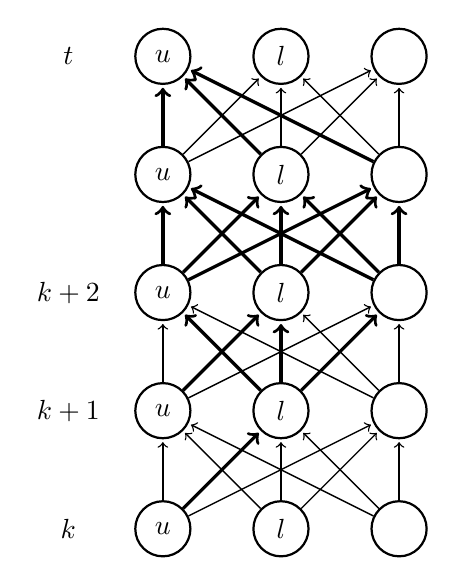
\begin{tikzpicture}[rnn_style]

  
  \node[neuron]    (x1)[]   {$u$};
  \node[neuron]    (x2)[right of=x1]   {$l$};
  \node[neuron]    (x3)[right of=x2]   {};
  \node[label]     (xl)[left of=x1] {$t$};
  
  \node[neuron]    (h1)[below of =x1]   {$u$};
  \node[neuron]    (h2)[right of=h1]   {$l$};
  \node[neuron]    (h3)[right of=h2]   {};
  \node[label]     (hl)[left of=h1] {$\hdots$};
  
  \node[neuron]    (y1)[below of=h1]   {$u$};
  \node[neuron]    (y2)[right of=y1]   {$l$};
  \node[neuron]    (y3)[right of=y2]   {};
  \node[label]     (yl)[left of=y1] {$k+2$};

  
  \node[neuron]    (z1)[below of=y1]   {$u$};
  \node[neuron]    (z2)[right of=z1]   {$l$};
  \node[neuron]    (z3)[right of=z2]   {};
  \node[label]     (zl)[left of=z1] {$k+1$};
  
  \node[neuron]    (w1)[below of=z1]   {$u$};
  \node[neuron]    (w2)[right of=w1]   {$l$};
  \node[neuron]    (w3)[right of=w2]   {};
  \node[label]     (wl)[left of=w1] {$k$};

  
%   \node[label]      (lu)[left of=u] {$u$};
%   \node[label]      (ll)[left of=z1] {$l$};


  \path[->] (h1) edge [thick_edge]  (x1)
	    (h1) edge [thin_edge]   (x2)
	    (h1) edge [thin_edge]   (x3)
	    (h2) edge [thick_edge]  (x1)
	    (h2) edge [thin_edge]   (x2)
	    (h2) edge [thin_edge]   (x3)
	    (h3) edge [thick_edge]  (x1)
	    (h3) edge [thin_edge]   (x2)
	    (h3) edge [thin_edge]   (x3);

  \path[->] (y1) edge [thick_edge]   (h1)
	    (y1) edge [thick_edge]   (h2)
	    (y1) edge [thick_edge]   (h3)
	    (y2) edge [thick_edge]   (h1)
	    (y2) edge [thick_edge]   (h2)
	    (y2) edge [thick_edge]   (h3)
	    (y3) edge [thick_edge]   (h1)
	    (y3) edge [thick_edge]   (h2)
	    (y3) edge [thick_edge]   (h3);
  
  
  \path[->] (z1) edge [thin_edge]   (y1)
	    (z1) edge [thick_edge]  (y2)
	    (z1) edge [thin_edge]   (y3)
	    (z2) edge [thick_edge]  (y1)
	    (z2) edge [thick_edge]  (y2)
	    (z2) edge [thick_edge]  (y3)
	    (z3) edge [thin_edge]   (y1)
	    (z3) edge [thin_edge]   (y2)
	    (z3) edge [thin_edge]   (y3);
	    
  \path[->] (w1) edge [thin_edge]   (z1)
	    (w1) edge [thick_edge]  (z2)
	    (w1) edge [thin_edge]   (z3)
	    (w2) edge [thin_edge]   (z1)
	    (w2) edge [thin_edge]   (z2)
	    (w2) edge [thin_edge]   (z3)
	    (w3) edge [thin_edge]   (z1)
	    (w3) edge [thin_edge]   (z2)
	    (w3) edge [thin_edge]   (z3);

	    


\end{tikzpicture}
\caption{Nodes involved in $\frac{\partial a^t_u }{\partial a^k_l}$}
\label{deriv_arcs_rnn}
\end{figure}

In matrix notation we have:

\begin{equation}
 \frac{\partial \vec{a}^t}{\partial \mat{W}^{rec}} = \sum_{k=1}^t \frac{\partial \vec{a}^t}{\partial \vec{a}^k} \cdot \frac{\partial \vec{a}^k}{\partial \mat{W}^{rec}}
\end{equation}


\begin{equation}
\frac{\partial a^{k}}{\partial \mat{W}_j^{rec}} =
 \begin{bmatrix}
   \phi_1^{k-1}    & 0                & \cdots      & \cdots       & 0  \\
   0               & \phi_2^{k-1}     & \cdots      & \cdots       & 0  \\
   \vdots          & \vdots           & \ddots      & \vdots       &\vdots\\
   0               & \cdots           & \cdots      & \cdots       & \phi^{k-1}_{r}
\end{bmatrix}
\end{equation}

\begin{equation}
\triangleq \mat{\Delta}^{tk}
\end{equation}

\begin{align}
\mat{\Delta}^{tk} &= \mat{\Delta}^{t(k+1)} \cdot diag(\sigma'(\vec{a}^k)) \cdot \mat{W}^{rec} \\
&= \prod_{i=t-1}^{k} diag(\sigma'(\vec{a}^i)) \cdot \mat{W}^{rec}
\label{rnn_delta}
\end{align}

The derivatives with respect to $\mat{W}^{in}$ and $\vec{b}^{rec}$ have the same structure.
The derivatives with respect to $W^{out}, b^{out}$ are straightfoward:

\begin{equation}
\frac{\partial \vec{g}}{\partial \mat{W}^{out}} = \sum_{t=1}^T \frac{\partial g_t}{\partial \vec{y^t}} \cdot J(F) \cdot \frac{\partial \vec{y}^t}{\partial \mat{W}^{out}} 
\end{equation}

\begin{equation}
\frac{\partial \vec{g}}{\partial \vec{b}^{out}} = \sum_{t=1}^T \frac{\partial g_t}{\partial \vec{y^t}} \cdot J(F) \cdot \frac{\partial \vec{y}^t}{\partial \vec{b}^{out}} 
\end{equation}

\paragraph{Backpropagation through time (BPTT)}
\textit{Backpropagation through time} is an extension of the \textit{backpropagation} algorithm we described for FNNs, we can think of BPTT
simply as a standard BP in the unfolded network. The same consideration done for BP also apply for BPTT, the difference is of course in how derivatives
are computed, equation \ref{rnn_delta}. Time complexity is easily derived noticing that in the unfolded network there are $n \cdot T$ units, where $n$ is the number of units of the RNN .This
yields time complexity $\mathcal{O}(\mathcal{N}(\set{W})\cdot T)$. Please see \cite{Williams90anefficient} for more details.












